\documentclass[aspectratio=169]{beamer}
\usepackage{tikz}
\usepackage{graphicx}
\usepackage{listings}
\usepackage{xcolor}
\usepackage{hyperref}
\usepackage[spanish,es-noquoting]{babel}

\lstset{
  basicstyle=\ttfamily\small,
  keywordstyle=\color{blue},
  stringstyle=\color{red},
  commentstyle=\color{gray},
  showstringspaces=false
}
% Minimal look
\usetheme{Warsaw}
%\setbeamertemplate{headline}
\setbeamertemplate{footline}{
  \leavevmode%
  \hbox{%
    % Left: Section name
    \begin{beamercolorbox}[wd=.33\paperwidth,ht=2.25ex,dp=1ex,left]{author in head/foot}%
      \hspace*{2ex}\insertsection
    \end{beamercolorbox}%
    % Center: Presentation title
    \begin{beamercolorbox}[wd=.34\paperwidth,ht=2.25ex,dp=1ex,center]{title in head/foot}%
      \insertshorttitle
    \end{beamercolorbox}%
    % Right: Slide numbers
    \begin{beamercolorbox}[wd=.33\paperwidth,ht=2.25ex,dp=1ex,right]{date in head/foot}%
      \insertframenumber{} / \inserttotalframenumber\hspace*{2ex}
    \end{beamercolorbox}%
  }%
  \vskip0pt%
}

\usecolortheme{default}
\usefonttheme{serif}
\graphicspath{{../}{./}}
\setbeamertemplate{caption}[numbered]

% Title info
\title[ IA y Derecho]{ IA y Derecho: Todo lo que necesitas saber antes de empezar}
\subtitle{ De Modelos Fundacionales a Estrategia Legal (Módulo 1)}
\author{Ricardo Reyes-Jimenez}
\institute{Universidad de La Sabana}
\date{\today}

% Background image for title slide
\usebackgroundtemplate{
  \tikz\node[opacity=0.3]{
\includegraphics[width=\paperwidth,height=\paperheight]{Images/UniSabana.jpg}};
}

\begin{document}

% Title slide
\begin{frame}
  \titlepage
\end{frame}

% Reset background for normal slides
\usebackgroundtemplate{}


\begin{frame}{Objetivos de la Sesión}
\begin{itemize}
  \item Entender la arquitectura tecnológica moderna (2026): IA Generativa vs Tradicional.
  \item Orquestación: Por qué las plataformas legales usan múltiples modelos a la vez.
  \item Adopción real: Qué funciona hoy en Colombia y el mundo.
  \item Casos de uso inmediatos y herramientas clave (Harvey, Lexis+AI, Claude, etc.).
  \item Gestión de Riesgos: Privacidad y Propiedad Intelectual.
\end{itemize}
\end{frame}


\begin{frame}{Desmitificando la Tecnología (El ``Matryoshka'' de la IA)}
\textbf{Conceptos Fundamentales:}
\begin{itemize}
  \item \textbf{Inteligencia Artificial (IA):} Máquinas replicando capacidades cognitivas.
  \item \textbf{Machine Learning \& Deep Learning:} Aprendizaje a partir de datos históricos mediante redes neuronales.
  \item \textbf{IA Generativa y LLMs (Large Language Models):} Modelos estadísticos avanzados que predicen lenguaje. No ``piensan'' como abogados, calculan probabilidades semánticas.
\end{itemize}
\end{frame}


\begin{frame}{El ``Matryoshka'' de la IA (Visual)}
\begin{figure}\centering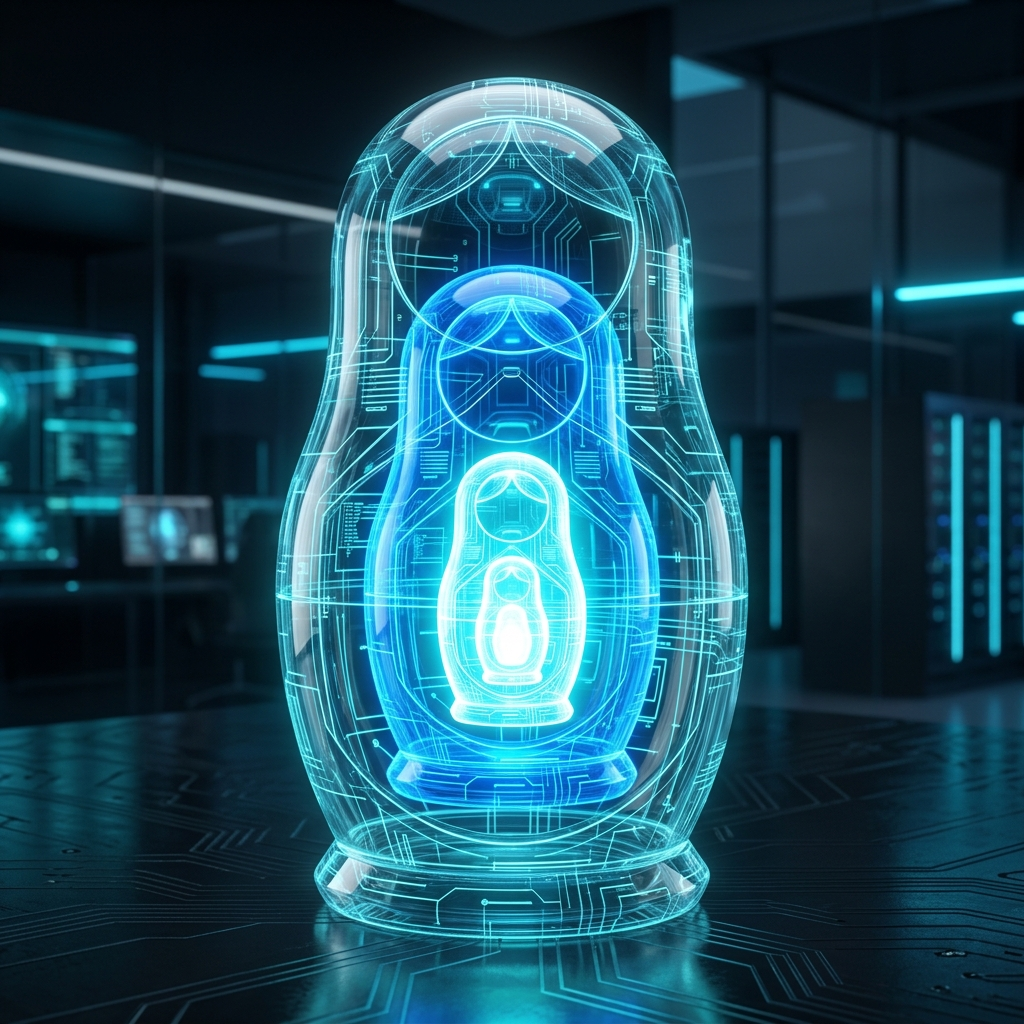
\includegraphics[height=0.6\textheight,keepaspectratio]{Images/matryoshka_ai_1785900912673.png}\caption{Matryoshka de la IA}\end{figure}
\end{frame}


\begin{frame}{Evolución 2026: De Modelos Solos a Sistemas Orquestados}
\textbf{¿Cómo funciona una plataforma LegalTech de alto nivel (ej. Harvey o Lexis+AI)?}
\begin{itemize}
  \item \textbf{No es un solo modelo:} No le hablan a un único 'cerebro'.
  \item \textbf{Sistemas Multi-Modelo:} Hay un modelo que lee tu pregunta (Router), otro especializado en extraer leyes, otro en razonar el caso, y otro que redacta el texto final.
  \item \textbf{RAG (Generación Aumentada por Recuperación):} La IA consulta la base de datos de jurisprudencia de la firma \textit{antes} de responder, eliminando alucinaciones \cite{relativity2024}.
\end{itemize}
\end{frame}


\begin{frame}{Automatización vs. Inteligencia Artificial}
\textbf{El Cambio en el Despacho}
\begin{itemize}
  \item \textbf{RPA (Tradicional):} Macros, flujos rígidos. (`SI A $\rightarrow$ ENTONCES B`). Falla si el documento cambia.
  \item \textbf{IA Generativa:} Interpreta contexto. Puede leer un correo furioso, entender la intención, y redactar una respuesta conciliatoria.
\end{itemize}
\end{frame}


\begin{frame}{RPA vs IA Generativa (Visual)}
\begin{figure}\centering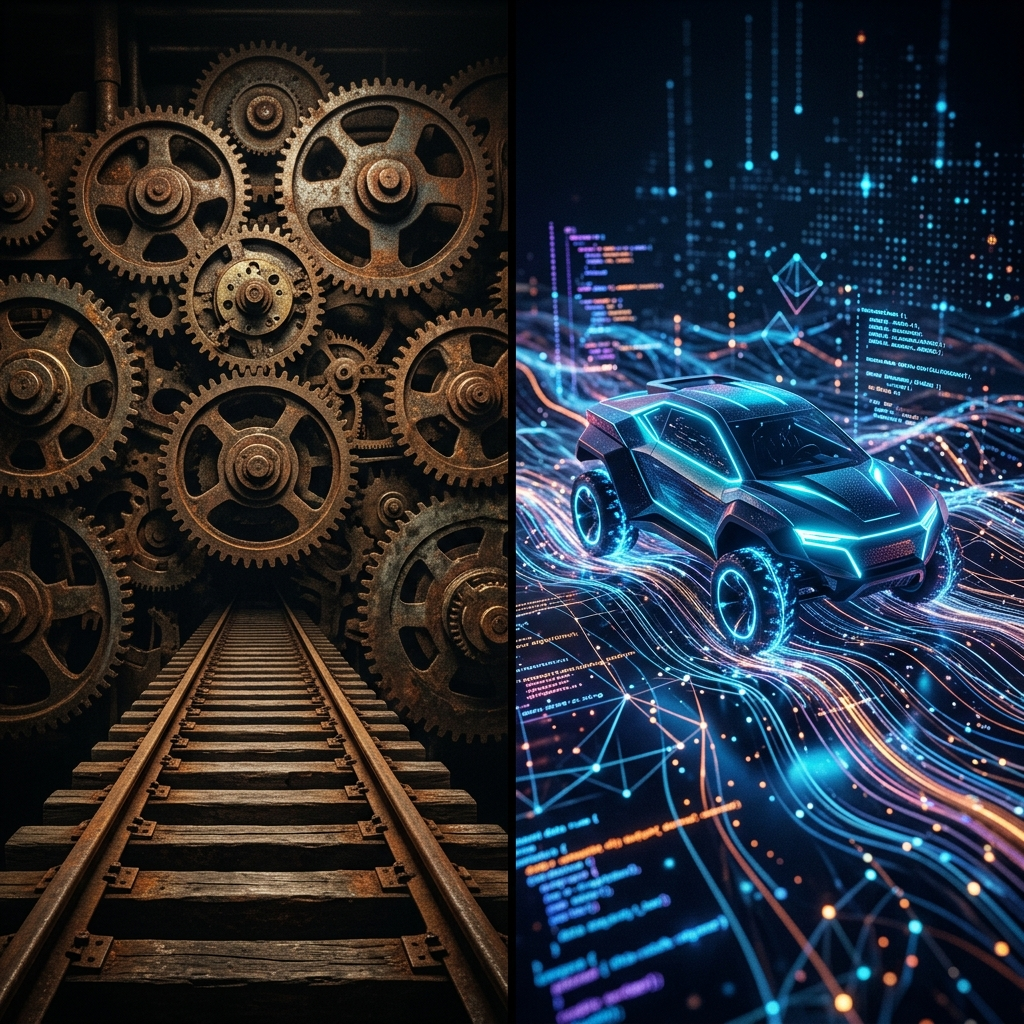
\includegraphics[height=0.6\textheight,keepaspectratio]{Images/rpa_vs_genai_1785900922553.png}\caption{RPA vs IA Generativa}\end{figure}
\end{frame}


\begin{frame}{Casos de Uso de Alto Impacto y Herramientas (2026)}
\begin{table}
\resizebox{\textwidth}{!}{
\begin{tabular}{|l | l | l | l|}
\hline
\textbf{Herramienta} & \textbf{Caso de Uso Principal} & \textbf{Sitio Web} & \textbf{Referencia} \\ \hline
Harvey AI & Investigación y Análisis Complejo & \href{https://www.harvey.ai/}{harvey.ai} & \cite{harvey2024} \\ \hline
Lexis+ AI & Investigación Jurídica y Jurisprudencia & \href{https://www.lexisnexis.com/en-us/products/lexis-plus-ai.page}{lexisnexis.com} & \cite{lexis2024} \\ \hline
Luminance & Due Diligence y Revisión de Contratos & \href{https://www.luminance.com}{luminance.com} & \cite{luminance2024} \\ \hline
vLex & Inteligencia Legal Global y Derecho Comparado & \href{https://vlex.com}{vlex.com} & \cite{vlex2024} \\ \hline
CoCounsel & Asistente Legal Integrado (Casetext/TR) & \href{https://legal.thomsonreuters.com/en/casetext}{casetext.com} & \cite{cocounsel2024} \\ \hline
Spellbook & Redacción y Revisión en Microsoft Word & \href{https://www.spellbook.legal}{spellbook.legal} & \cite{spellbook2024} \\ \hline
Clearbrief & Verificación de Hechos y Escritos Judiciales & \href{https://clearbrief.com}{clearbrief.com} & \cite{clearbrief2024} \\ \hline
Relativity aiR & E-Discovery y Revisión Documental Masiva & \href{https://www.relativity.com/data-solutions/ai/}{relativity.com} & \cite{relativityair2024} \\ \hline
Everlaw & Gestión de Litigios e Investigaciones & \href{https://www.everlaw.com}{everlaw.com} & \cite{everlaw2024} \\ \hline
Ironclad AI & Gestión del Ciclo de Vida de Contratos (CLM) & \href{https://ironcladapp.com}{ironcladapp.com} & \cite{ironclad2024} \\ \hline
\end{tabular}
}
\end{table}
\end{frame}


\begin{frame}{Adopción Real: Colombia y el Resto del Mundo}
\begin{itemize}
  \item \textbf{Tendencia Global:} Las firmas ya no evalúan ``si'' usar IA, sino ``cómo'' integrarla en flujos (Word, Teams) y medir el ROI \cite{thomsonreuters2024}.
  \item \textbf{Colombia / LatAm:} Transición de pilotos a infraestructura base. Los clientes empiezan a exigir eficiencias basadas en IA en la facturación (Adiós al modelo de horas facturables en tareas repetitivas).
\end{itemize}
\end{frame}


\begin{frame}{La IA: ¿Amiga o Enemiga? (Visual)}
\begin{figure}\centering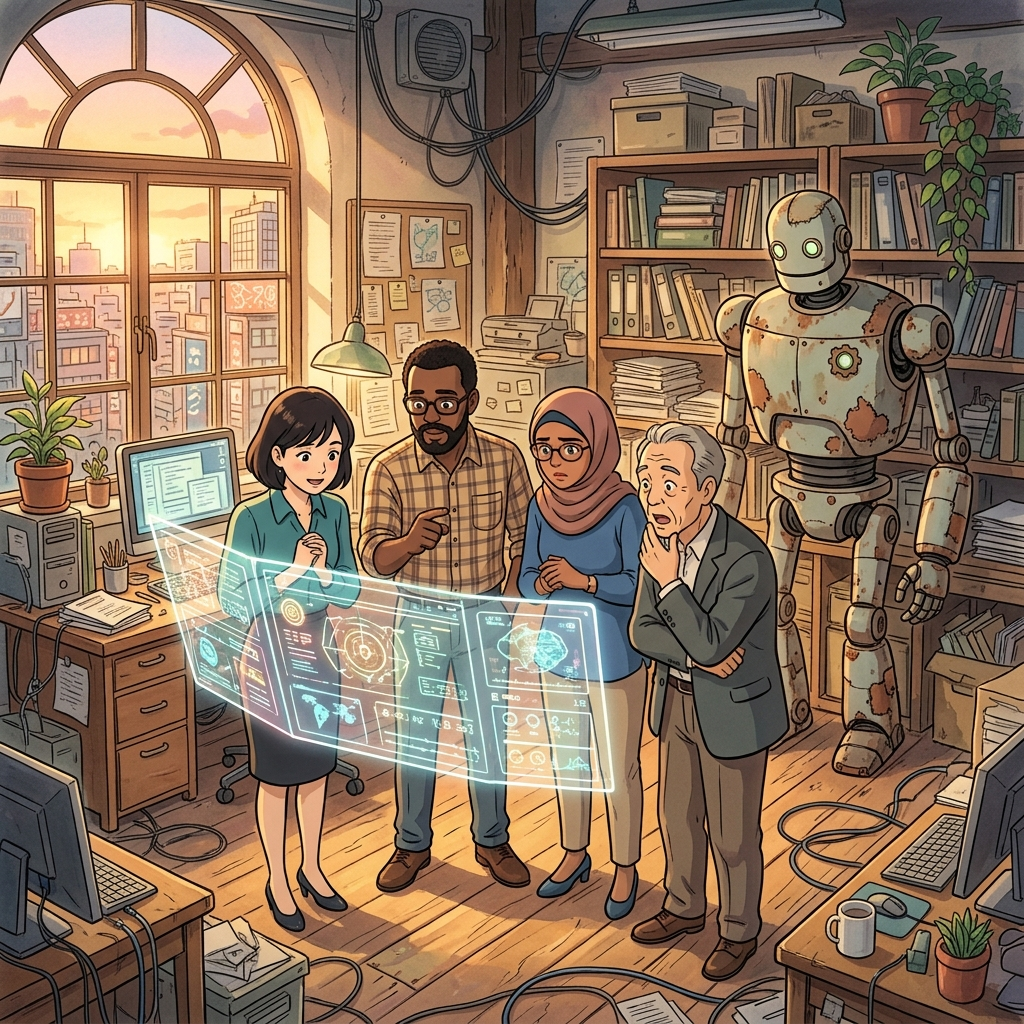
\includegraphics[height=0.6\textheight,keepaspectratio]{Images/ia_amiga_enemiga.png}\caption{IA en el Entorno Laboral}\end{figure}
\end{frame}


\begin{frame}{Gestión de Riesgos: Privacidad (Ley 1581)}
\begin{itemize}
  \item \textbf{El Error de Novato:} Subir contratos con datos personales a ChatGPT gratuito.
  \item \textbf{El Riesgo Inminente:} Transmisión internacional de datos no autorizada, violación de confidencialidad cliente-abogado.
  \item \textbf{Soluciones Empresariales:} Licencias ``Zero Data Retention'' (Copilot Enterprise, Claude Team, Harvey). Sus datos no entrenan al modelo público.
\end{itemize}
\end{frame}


\begin{frame}{Bóveda de Privacidad (Visual)}
\begin{figure}\centering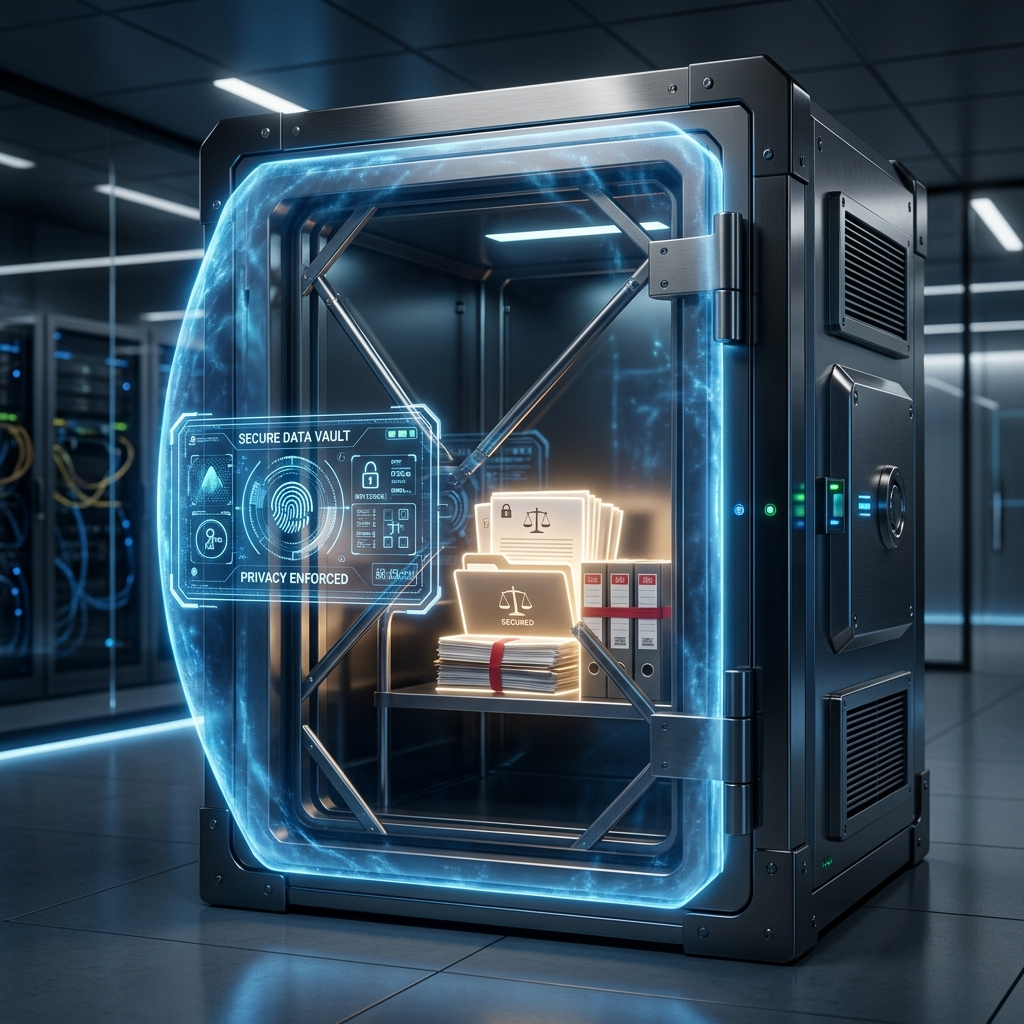
\includegraphics[height=0.6\textheight,keepaspectratio]{Images/privacy_vault_1785900930775.png}\caption{Bóveda de Privacidad Zero Data}\end{figure}
\end{frame}


\begin{frame}{Privacidad en Herramientas Gratuitas (Opt-Out)}
\textbf{Si su equipo usa cuentas gratuitas, la IA se entrena con sus datos por defecto.} Cómo desactivarlo:
\begin{itemize}
  \item \textbf{ChatGPT:} \textit{Settings} $\rightarrow$ \textit{Data Controls} $\rightarrow$ Apagar \textit{``Improve the model for everyone''}.
  \item \textbf{Claude:} \textit{Settings} $\rightarrow$ \textit{Privacy} $\rightarrow$ Apagar \textit{``Help improve Claude''}.
  \item \textbf{Gemini:} \textit{myactivity.google.com} $\rightarrow$ \textit{Gemini Apps Activity} $\rightarrow$ Seleccionar \textit{``Turn off''}.
\end{itemize}
\textbf{IMPORTANTE - ADVERTENCIA LEGAL (Ley 1581/2012):} Incluso con el \textit{Opt-Out}, subir Datos Personales o Secreto Profesional a entornos B2C gratuitos puede constituir una Transmisión Internacional de Datos no autorizada. La falta de debida diligencia conlleva severas sanciones de la SIC y violaciones a la ética profesional.
\end{frame}


\begin{frame}{Riesgos: Propiedad Intelectual y 'Alucinaciones'}
\begin{itemize}
  \item \textbf{Derechos de Autor (DNDA):} El producto de la IA no es protegible por derecho de autor sin intervención humana sustancial.
  \item \textbf{Human-in-the-Loop:} La IA no reemplaza la responsabilidad ética y civil del abogado. La supervisión es obligatoria.
\end{itemize}
\end{frame}


\begin{frame}{Los Desafíos de la IA (Visual)}
\begin{figure}\centering
\includegraphics[height=0.6\textheight,keepaspectratio]{Images/desafios_ia.png}\caption{Desafíos y Auditoría de la IA}\end{figure}
\end{frame}


\begin{frame}{Taller de Cierre: La Política de IA de su Firma}
\begin{itemize}
  \item \textbf{Actividad en Grupos:} Diseñar los 3 pilares de la política de uso de IA para sus equipos (Qué se permite, qué herramientas, y qué flujos de revisión).
  \item \textbf{Debrief \& Mentoría.}
\end{itemize}
\end{frame}



\begin{frame}[allowframebreaks]{Referencias}
  \bibliographystyle{apalike}
  \bibliography{references}
\end{frame}

\end{document}